%% Author=Danny Kaplan
%% Date=Dec 3, 2010
%% Subject=Derivatives
%% RelatesTo=Optimization
\begin{knitrout}
\definecolor{shadecolor}{rgb}{0.969, 0.969, 0.969}\color{fgcolor}\begin{kframe}


{\ttfamily\noindent\color{warningcolor}{\#\# Warning in file(filename, "{}r"{}, encoding = encoding): cannot open file '/../../../Public/math135.R': No such file or directory}}

{\ttfamily\noindent\bfseries\color{errorcolor}{\#\# Error in file(filename, "{}r"{}, encoding = encoding): cannot open the connection}}

{\ttfamily\noindent\bfseries\color{errorcolor}{\#\# Error in eval(expr, envir, enclos): object '..' not found}}\end{kframe}
\end{knitrout}

\SweaveOpts{prefix.string=Figures/tradeoffs,keep.source=TRUE}

In budgeting for health-care,  policy makers need to decide what are
the best ways to spend the available funds.  One way for analyzing the
possibilities involves examining the impact of spending the money in
different ways, measured by ``Quality Adjusted Life Years,'' QALYs.

Suppose that each year, vaccinations given to children save 100
lives.  Since children can be expected to live another 70 years or so,
those vaccinations would be credited with $70 \times 100$ life years.
The point of ``quality adjusted'' is to take into account that many
health interventions preserve the lives of people who have substantial
disability or distress.

The graph below shows a hypothetical situation of three different
interventions, labelled A, B, and C.  Each curve shows the number of
QALYs that would result from spending the indicated amount of money.
By spending more money on an intervention, you can reach more people
or produce a better outcome for those people who are reached.  



\centerline{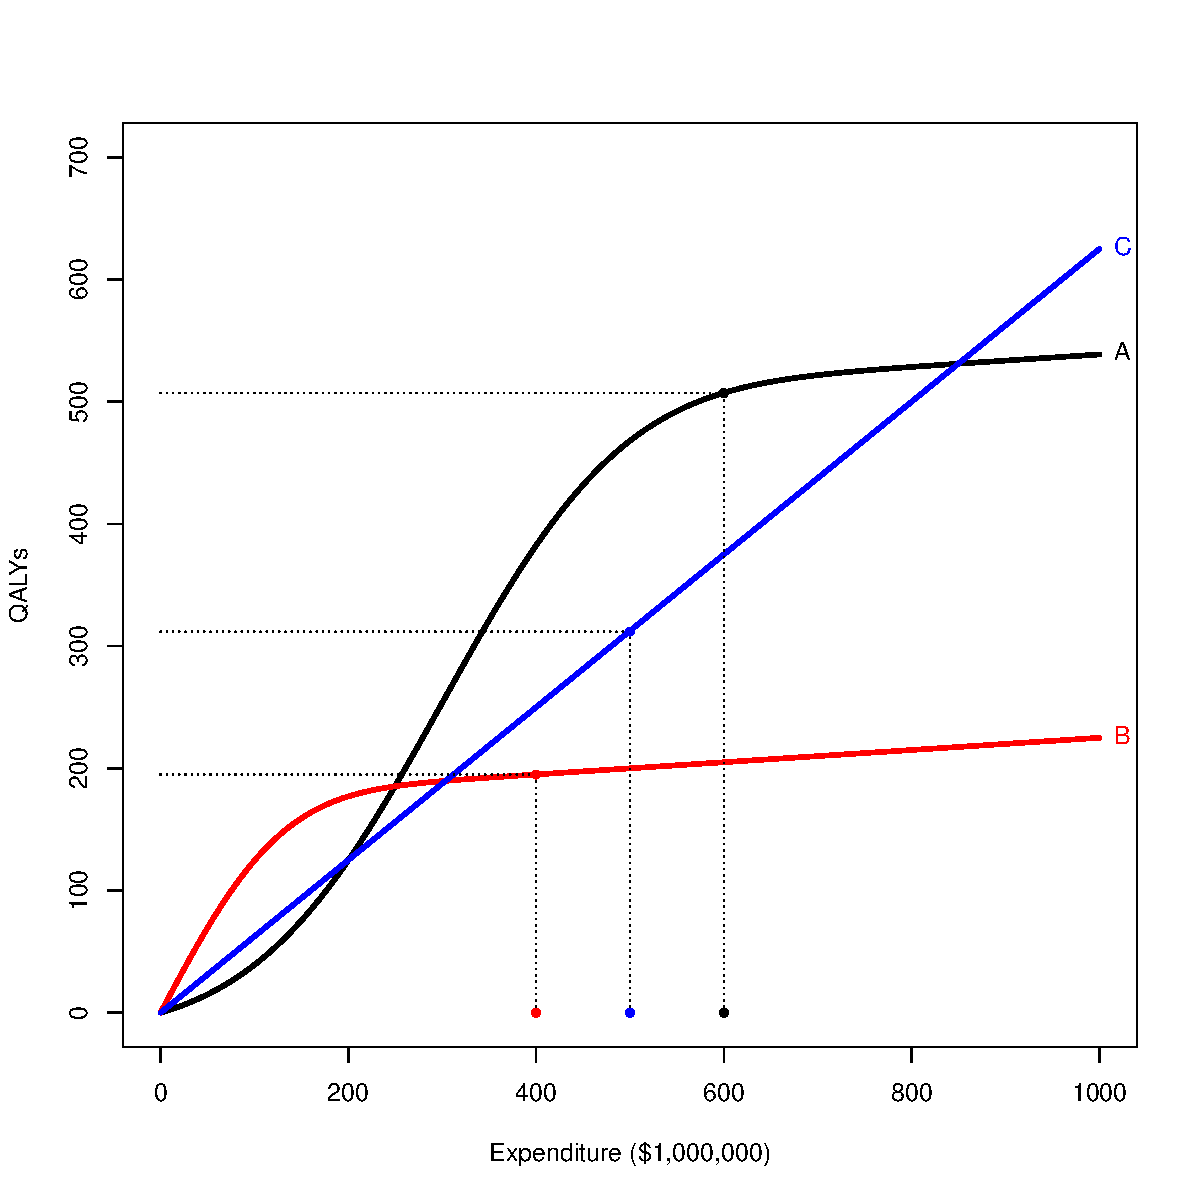
\includegraphics[width=5in]{Figures/tradeoffs-qaly1}}

The current health policy is indicated by the dots on each curve:
\$600 million for A, \$400 million for B, and \$500 million for C.
Notice that the money amounts add up to a total of \$1500 million.
That's the budget.

\newpage
\begin{enumerate}

\item At the money allocation policy shown in the graph, how many QALY's would
result for a \$1 million increase in funding for policy A?

\answerSpace{1in}


\item If you had to cut the budget by \$1 million, which single intervention, A,
  B, or C,  would you reduce funding for?

\answerSpace{1in}

\item Give an allocation policy that improves the total number of QALYs, summed
across the three interventions, but stays within the total budget of
\$1500 million?  Explain the strategy that you used to find
the improved allocation?

\answerSpace{1.3in}

\item Give a general statement about what sort of allocation of money
  among A, B, and C would give the largest possible total number of
  QALYs, summed across the three interventions, and staying within the
  total budget of \$1500 million.

\answerSpace{1.3in}

\end{enumerate}
